\documentclass[14pt, a4paper]{report}
\usepackage{mathtext}
\usepackage[T2A]{fontenc}
\usepackage[utf8]{inputenc}
\usepackage[russian]{babel}
\usepackage{multirow}
\usepackage{slashbox}
\usepackage{makecell}
\usepackage{graphicx}
\usepackage{physics}
\usepackage{amstext}
\usepackage{caption}
\usepackage{subcaption}

\renewcommand{\thesection}{\arabic{section}.}
\renewcommand{\thesubsection}{\arabic{section}.\arabic{subsection}.}

\title{\textbf{Отчет о выполнении лабораторной работы 3.4.2 "Закон Кюри-Вейсса"}}
\author{Алпатова Александра и Калашников Михаил, Б03-205}
\date{}

\begin{document}
	\maketitle
	
	\textbf{Цель работы:}
	изучение температурной зависимости магнитной восприимчивости ферромагнетика выше точки Кюри.
	\newline
	
	\textbf{В работе используются:}
	\begin{itemize}
		\item катушка самоиндукции с образцом из гадолиния;
		\item термостат;
		\item частотомер;
		\item цифровой вольтметр;
		\item LC-автогенератор;
		\item термопара медь–константан.
	\end{itemize}
	
	\section{Теоретические сведения}
	
	
	
	\section{Экспериментальная установка}
	
	
	
	\section{Подготовка приборов к работе}
	
		\begin{enumerate}
		
			\setcounter{enumi}{0}
			
			\item Перед началом работы термостат был предварительно охлажден до $14^\circ C$.
	
			\item Включим в сеть автогенератор, частотометр GFC-8010 и вольтметр B7-78.
	
			\item Для обеспечения требуемой точности измерений, рассчитаем при каком показании вольтметра температура термостата и образца отличаются на $\Delta T=0.5^\circ C$:
			\[U_0=\frac{\Delta T}{\kappa}=\frac{0.5^\circ C}{24\ \frac{^\circ C}{мВ}}\approx0.02\ мВ\]
			При дальнейшем нагревании термостата будем дожидаться пока показания вольтметра 
снизятся до $U_0$.

		\end{enumerate}

	\section{Проведение измерений}	

		\begin{enumerate}
		
			\setcounter{enumi}{3}

			\item Начнем постепенно нагревать термостат до $\ ^\circ C$, фиксируя показания приборов каждые $2\ ^\circ C$ и занося их в таблицу 1.
			Период колебаний без образца равен $\tau_0=9.045\ мкс$.
	
			\item Закончив измерения, отключим все приборы.
		
		\end{enumerate}

	\section{Обработка данных}

		\begin{enumerate}
		
			\setcounter{enumi}{5}

			\item Рассчитаем температуру образца с учетом показаний термостата по формуле: $T=T_{exp}+\kappa U$. Построим графики $(\tau^2-\tau_0^2)=f(T)$ (рис. 1) и $1/(\tau^2-\tau_0^2)=f(T)$ (рис. 2). Аппроксимируем первый график гиперболой и найдем на нем точку Кюри гадолиния.
			\[\Theta=284.4\pm0.8\ К\]
			На втором графике проведем прямую МНК через точки, начиная с пятой -- с этого момента зависимость выходит на асимптоту. Найдем парамагнитную точку Кюри $\Theta_p$ как пересечение данной прямой и оси абсцисс.
			\[\Theta_p=291\pm9\ К\]

		\end{enumerate}
	
	\section{Приложения}
	
		\begin{figure}[h]
			\centering
			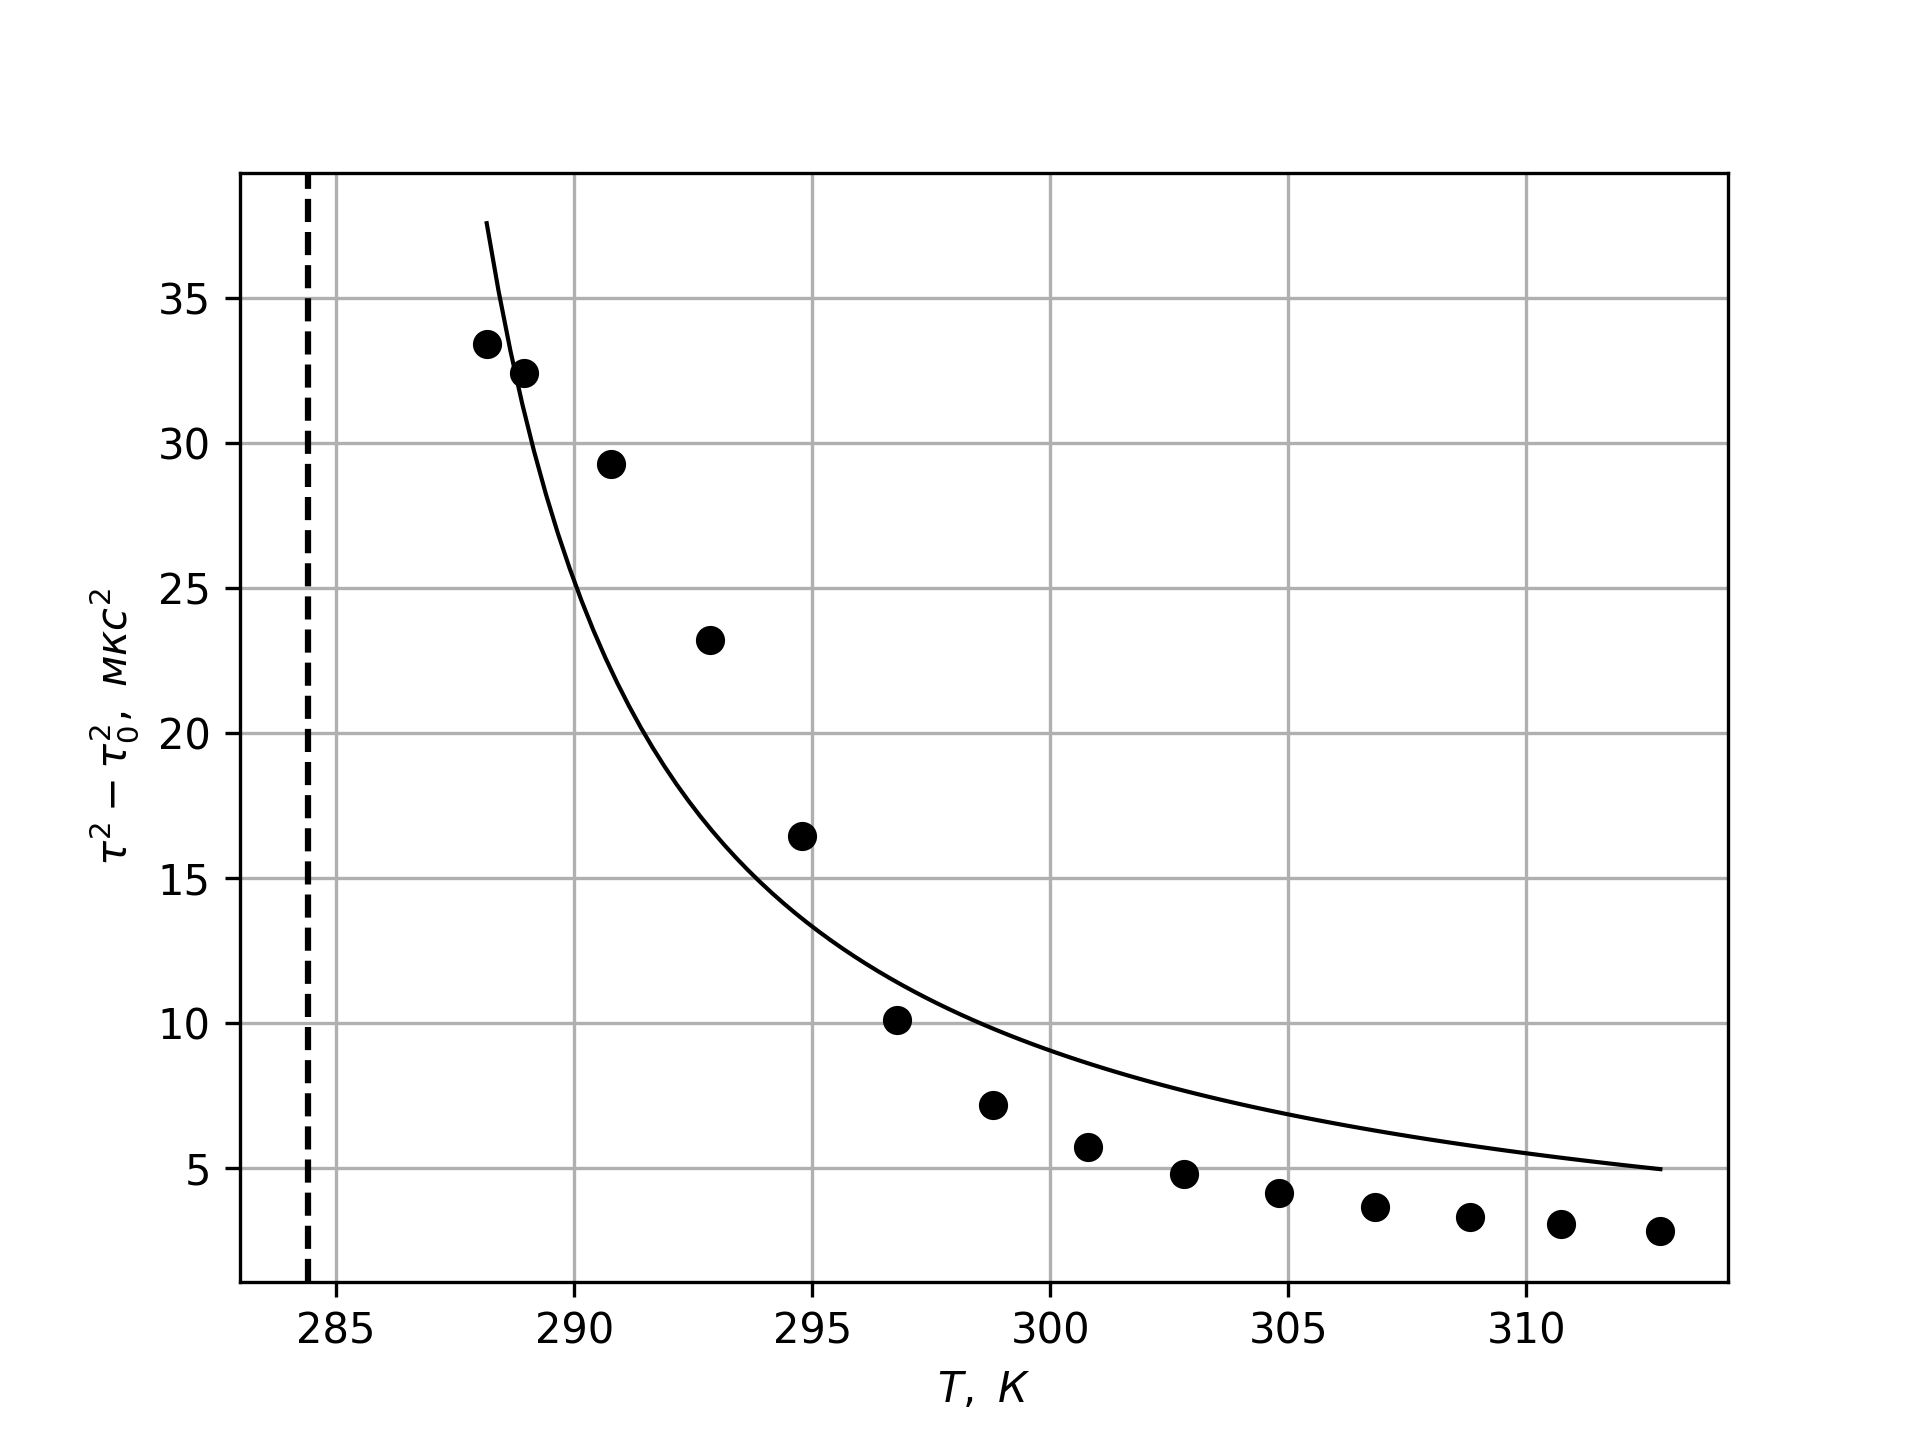
\includegraphics[width=0.75\linewidth]{images/342_1.png}
			\caption{График зависимости $(\tau^2-\tau_0^2)=f(T)$}
		\end{figure}

		\begin{figure}[h]
			\centering
			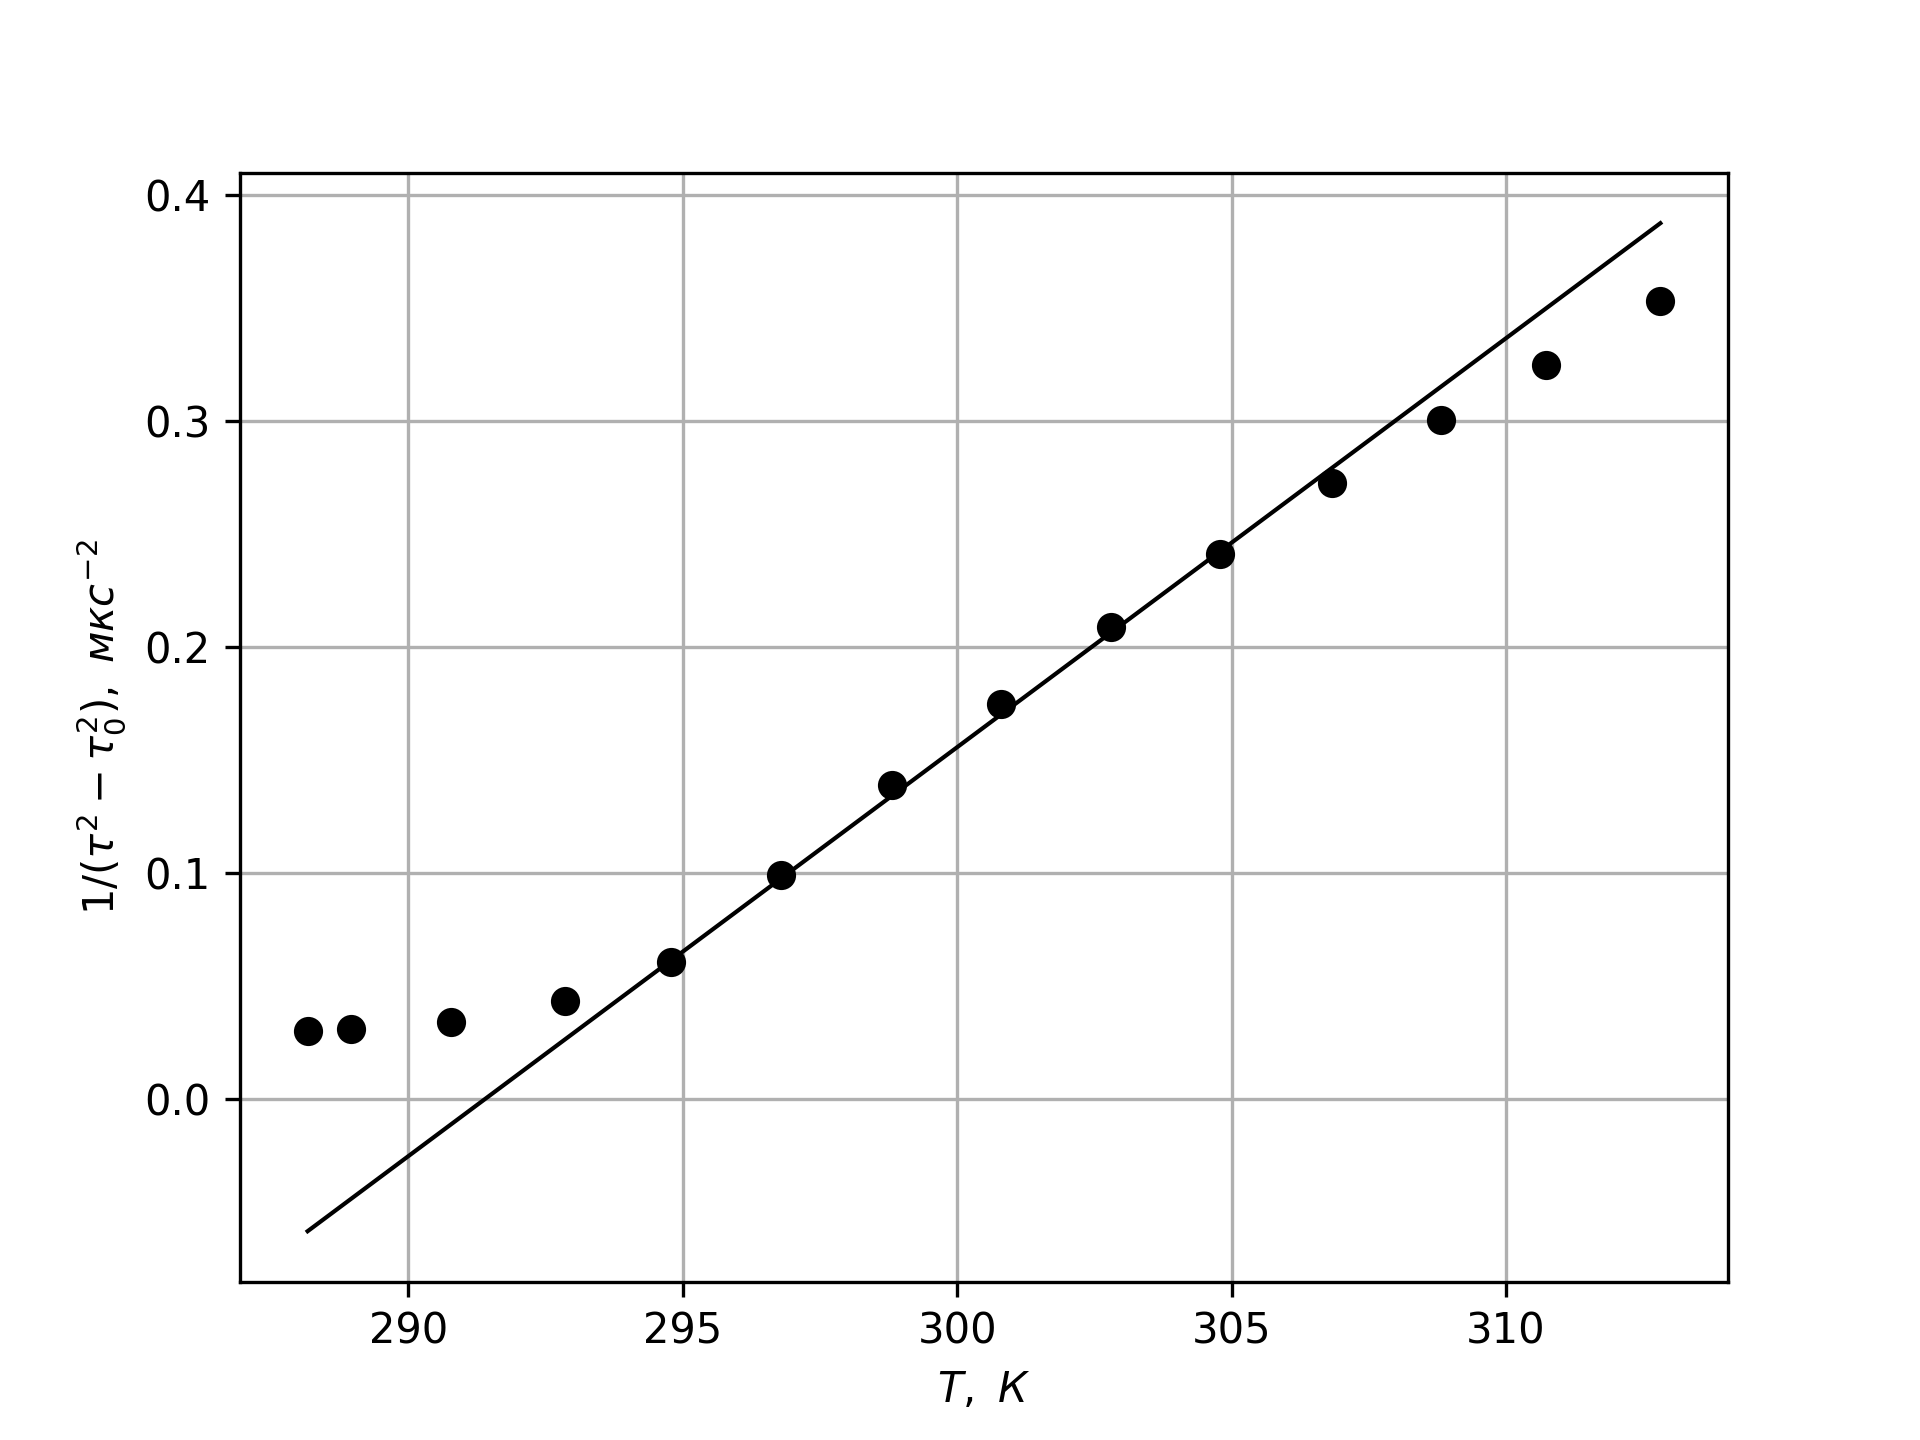
\includegraphics[width=0.75\linewidth]{images/342_2.png}
			\caption{График зависимости $1/(\tau^2-\tau_0^2)=f(T)$}
		\end{figure}

\end{document}